%
% kubisch.tex
%
% (c) 2018 Prof Dr Andreas Müller, Hochschule Rapperswil
%
\documentclass[tikz]{standalone}
\usepackage{times}
\usepackage{amsmath}
\usepackage{txfonts}
\usepackage[utf8]{inputenc}
\usepackage{graphics}
\usetikzlibrary{arrows,intersections,math}
\begin{document}

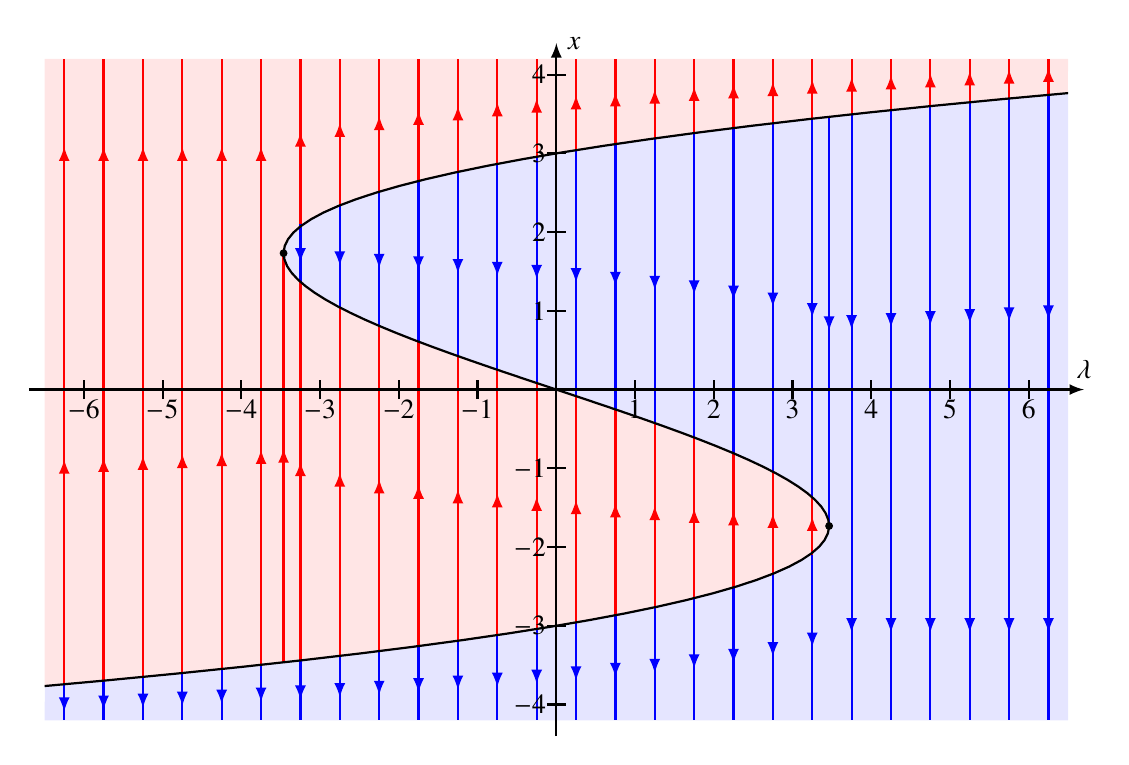
\begin{tikzpicture}[>=latex,thick]

\def\w{6.5}
\def\h{4.2}
\def\s{0.12}

\tikzmath {
	real \xupper, \xlower, \l;
	\l = \w;
	\xupper = \h;
	\x = \xupper;
	\x = \x - ((\x*\x - 9) * \x - 3 * \l) / (3*\x*\x - 9);
	\x = \x - ((\x*\x - 9) * \x - 3 * \l) / (3*\x*\x - 9);
	\x = \x - ((\x*\x - 9) * \x - 3 * \l) / (3*\x*\x - 9);
	\x = \x - ((\x*\x - 9) * \x - 3 * \l) / (3*\x*\x - 9);
	\xupper = \x;
	\xlower = -\xupper;
}

\fill[color=red!10,domain={\xlower}:{\xupper},samples=100]
	({\w},{\h})--({-\w},{\h})--({-\w},{\xlower})
	--plot ({(1/3)*\x*(\x*\x-9)},{\x})--cycle;
\fill[color=blue!10,domain={\xupper}:{\xlower},samples=100]
	({-\w},{-\h})--({\w},{-\h})--({\w},{\xupper})
	--plot ({(1/3)*\x*(\x*\x-9)},{\x})--cycle;

\tikzmath {
	real \xupper, \xmax, \xmiddle, \l;
	\l = 2 * sqrt(3);
	\xupper = 2 * sqrt(3);
	\xmax = -sqrt(3);
	\xmiddle = (\xupper + \xmax)/2;
}

\draw[->,color=blue] ({\l},{\xupper})--({\l},{\xmiddle-\s});
\draw[color=blue] ({\l},{\xmiddle})--({\l},{\xmax});
\draw[->,color=red] ({-\l},{-\xupper})--({-\l},{-\xmiddle+\s});
\draw[color=red] ({-\l},{-\xmiddle})--({-\l},{-\xmax});

\fill ({\l},{\xmax}) circle[radius=0.05];
\fill ({-\l},{-\xmax}) circle[radius=0.05];

\foreach \l in {-3.25,-2.75,...,3.25}{
	\tikzmath {
		real \xupper, \xlower, \xmiddle;
		\xupper = \h;
		\x = \xupper;
		\x = \x - ((\x*\x - 9) * \x - 3 * \l) / (3*\x*\x - 9);
		\x = \x - ((\x*\x - 9) * \x - 3 * \l) / (3*\x*\x - 9);
		\x = \x - ((\x*\x - 9) * \x - 3 * \l) / (3*\x*\x - 9);
		\x = \x - ((\x*\x - 9) * \x - 3 * \l) / (3*\x*\x - 9);
		\xupper = \x;
		\xmiddle = 0;
		\x = \xmiddle;
		\x = \x - ((\x*\x - 9) * \x - 3 * \l) / (3*\x*\x - 9);
		\x = \x - ((\x*\x - 9) * \x - 3 * \l) / (3*\x*\x - 9);
		\x = \x - ((\x*\x - 9) * \x - 3 * \l) / (3*\x*\x - 9);
		\x = \x - ((\x*\x - 9) * \x - 3 * \l) / (3*\x*\x - 9);
		\xmiddle = \x;
		\xlower = -\h;
		\x = \xlower;
		\x = \x - ((\x*\x - 9) * \x - 3 * \l) / (3*\x*\x - 9);
		\x = \x - ((\x*\x - 9) * \x - 3 * \l) / (3*\x*\x - 9);
		\x = \x - ((\x*\x - 9) * \x - 3 * \l) / (3*\x*\x - 9);
		\x = \x - ((\x*\x - 9) * \x - 3 * \l) / (3*\x*\x - 9);
		\xlower = \x;
	}

	\draw[->,color=red] ({\l},{\xupper})--({\l},{(\xupper+\h)/2+\s});
	\draw[color=red] ({\l},{(\xupper+\h)/2})--({\l},{\h});

	\draw[->,color=blue] ({\l},{\xupper})--({\l},{(\xupper+\xmiddle)/2-\s});
	\draw[color=blue] ({\l},{(\xupper+\xmiddle)/2})--({\l},{\xmiddle});

	\draw[->,color=red] ({\l},{\xlower})--({\l},{(\xlower+\xmiddle)/2+\s});
	\draw[color=red] ({\l},{(\xlower+\xmiddle)/2})--({\l},{\xmiddle});

	\draw[->,color=blue] ({\l},{\xlower})--({\l},{(\xlower-\h)/2-\s});
	\draw[color=blue] ({\l},{(\xlower-\h)/2})--({\l},{-\h});
}

\foreach \l in {3.75,4.25,...,6.25}{
	\tikzmath {
		real \xupper;
		\xupper = \h;
		\x = \xupper;
		\x = \x - ((\x*\x - 9) * \x - 3 * \l) / (3*\x*\x - 9);
		\x = \x - ((\x*\x - 9) * \x - 3 * \l) / (3*\x*\x - 9);
		\x = \x - ((\x*\x - 9) * \x - 3 * \l) / (3*\x*\x - 9);
		\x = \x - ((\x*\x - 9) * \x - 3 * \l) / (3*\x*\x - 9);
		\xupper = \x;
		real \xoben, \xunten;
		\xoben = (\xupper - sqrt(3)) / 2;
		\xunten = (-sqrt(3) - \h) / 2;
	}
	\draw[->,color=blue] ({\l},{\xupper})--({\l},{\xoben-\s});
	\draw[->,color=blue] ({\l},{\xoben})--({\l},{\xunten-\s});
	\draw[color=blue] ({\l},{\xunten})--({\l},{-\h});

	\draw[->,color=red] ({\l},{\xupper})--({\l},{(\xupper+\h)/2+\s});
	\draw[color=red] ({\l},{(\xupper+\h)/2})--({\l},{\h});

	\draw[->,color=red] ({-\l},{-\xupper})--({-\l},{-\xoben+\s});
	\draw[->,color=red] ({-\l},{-\xoben})--({-\l},{-\xunten+\s});
	\draw[color=red] ({-\l},{-\xunten})--({-\l},{\h});

	\draw[->,color=blue] ({-\l},{-\xupper})--({-\l},{-(\xupper+\h)/2-\s});
	\draw[color=blue] ({-\l},{-(\xupper+\h)/2})--({-\l},{-\h});
}

\begin{scope}
\clip ({-\w},{-\h}) rectangle ({\w},{\h});

\draw[domain={-\h}:{\h},samples=100] plot ({(1/3)*(\x*\x-9)*\x},{\x});

\end{scope}

\draw[->] ({-\w-0.2},0)--({\w+0.2},0) coordinate[label=$\lambda$];
\draw[->] (0,{-\h-0.2})--(0,{\h+0.2}) coordinate[label={right:$x$}];

\foreach \l in {-6,-5,-4,-3,-2,-1,1,2,3,4,5,6}{
	\draw ({\l},{-\s})--({\l},\s);
	\node at ({\l},0) [below] {$\l$};
}

\foreach \x in {-4,-3,-2,-1,1,2,3,4}{
	\draw ({-\s},{\x})--(\s,{\x});
	\node at (0,{\x}) [left] {$\x$};
}

\end{tikzpicture}

\end{document}
